\subsection{Long-slit spectroscopy mode}
\label{ssec:algo_lss_spectroscopy}

%-----------------------------------------------------------------------------------------
\subsubsection{Order background contamination removal}\label{ssec:orderbg}
Order background contamination may arise from internal straylight probably covering larger areas of the detector. Since it is expected to be low frequency only, its removal can be achieved by a low-order 2D polynomial fit 
\begin{equation}
    z = (a_0 + a_1x + a_2y + a_3x^2 + a_4x^2y + a_5x^2y^2 + a_6y^2 + a_7xy^2 + a_8xy ...)
\end{equation}
and a subsequent subtraction. The fitting points/regions must be chosen to be outside the \ac{LSS} order (cf. e.g. Figs~\ref{fig:ff}/\ref{fig:pinh} for simulated data). Whereas these fitting points/regions can be chosen on fairly regular basis due to the straight order geometry in the \ac{LSS} mode, the degree of the polynomial depends on the actual straylight. This can be determined only during the testing phase when first real data are available. Note that this algorithm will only be implemented in case such a contamination is visible.

%-----------------------------------------------------------------------------------------
\subsubsection{Order detection and rectification}\label{ssec:orderhandling}
The algorithms for order detection and rectification are adopted from~\cite{pis02,pis21}.
In brief, the selection of pixels that may belong to spectral \ac{LSS} order is done by first smoothing each column and then selecting pixels above the median of the difference between the original
and the smoothed column, i.e. pixel $(x,y)$ is selected if
\begin{equation}
    I(x,y) > \bar{I}(x,y) + \mathrm{Median} ( I(x,y) - \bar{I}(x,y) ) .
\end{equation}
In the following a clustering analysis is performed, which associates connected groups of pixels. This is done scanning rows and columns and identifying neighbouring pixels selected in the previous step as belonging to the same cluster if $\delta x$ and $\delta y$ differ by at most 1. As spectral orders may be partitioned into different clusters because of e.g. detector defects, polynomial fits to the clusters are performed and the pairwise extensions of the fits to consecutive clusters are compared to identify which clusters are to be merged according to predefined criteria for the goodness of match. For each order, the detection algorithm yields a polynomial description of order location on the detector (the order center and its edges), an uncertainty estimate
for the fitted polynomial, and the first and last columns to be used during spectrum extraction. 
%The upper and lower edges of the orders are also traced and fitted by the order tracing algorithm using the pinhole frames with the flatfield lamp. 
Order rectification is achieved using the PyReduce algorithm described by~\cite{pis21} that can account for both tilt and curvature of the slit image.   

%-----------------------------------------------------------------------------------------
\subsubsection{Wavelength calibration strategy}\label{ssec:wavecal}
The wavelength calibration (i.e. the pixel-to-wavelength relation) of the \ac{LSS} modes is done in a two-step approach:
\begin{itemize}
    \item First guess: The first guess is based on laser sources in the \ac{WCU} and during commissioning.  In the LM range, two fixed-frequency lasers ($@3.39$µm and $@5.26$µm) and one tuneable ($4.68....4.78$µm) is foreseen in the \ac{WCU} to be taken on daily basis (cf.~\cite{METIS-calibration_plan}). In the N-band, a laser source will only be available during \ac{AIT}. As we assume the instrument to be very stable, that approach should be sufficient to achieve a first guess solution for the low-resolution N-band spectroscopy.
    \item For the final calibration atmospheric lines are used in the recipes \REC{metis_LM_lss_sci} and \REC{metis_N_lss_sci}, which are used in the \texttt{pyreduce} package as reference frame.
    \item Optionally: the package \texttt{molecfit} in its newest version has a new function implemented, which allows a fine-tuning of the wavelength calibration by means of fitting atmospheric features. It is to be tested during commissioning, whether this step is required.
\end{itemize}

%-----------------------------------------------------------------------------------------
\subsubsection{Flux calibration / AO-induced slitlosses}\label{ssec:aoslitloss}
Similar to the MICAD instrument, we expect significant slit losses induced by the broad wings of the \ac{PSF}. In order get a first estimate we created a set of simulated \ac{SCAO}-\ac{PSF}s with \texttt{AnisoCado}\footnote{\url{https://anisocado.readthedocs.io/en/latest/}} incorporating three different turbulence profiles, the EsoMedian profile reflecting median conditions (seeing=0.67", $30^\circ$ zenith distance, wind speed 10\,m/s), and EsoQ1 and EsoQ4 representing the first (i.e. best) quartile of observing conditions (seeing=0.4", $0^\circ$ zenith distance, wind speed 8.8\,m/s), and the fourth (worst) quartile observing conditions  (seeing=1.0", $60^\circ$ zenith distance, wind speed 13\,m/s), respectively. For each turbulence profile, we calculated a set of \ac{PSF}s depending on the \ac{NGS} distance (varying between 0 and $20"\times20"$ with respect to the target position, cf. Fig.~\ref{fig:ngsoffsets}) and depending on the wavelength to cover the entire $L$, $M$, and $N$-bands with a wavelength step of 0.1$\mu$m. The size of the \ac{PSF}s were chosen to be $2048\times2048$ pixels.\\
Fig.~\ref{fig:scaopsfslits} shows as example the \ac{PSF} for the EsoMedian turbulence profile at $4.20\mu$m for an \ac{NGS}-distance of 0\arcsec (i.e. the best case when the science target star can be used as guide star) with the three slits. The flux losses were calculated as the fraction of the unity \ac{PSF} outside the slit area. The resulting slitlosses for the entire photometric bands for all slits are shown in Fig.~\ref{fig:slitlosses}.
\begin{figure}[ht!]
  \centering
  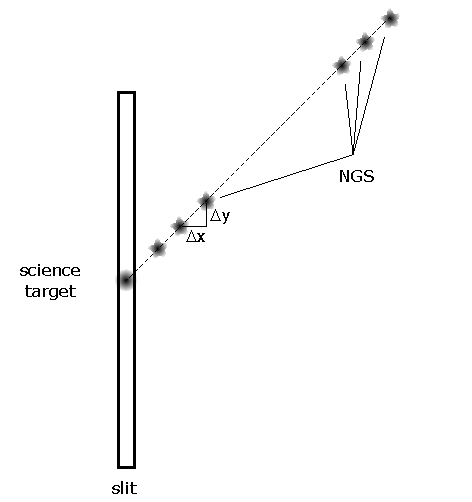
\includegraphics[width=0.5\linewidth]{figures/LSS_CrtAlg_files/ngs_offsets.pdf}
  \caption{Sketch of the used \ac{NGS} offsets ($\Delta x=\Delta y=1\arcsec$) with respect to the science target and the slits}
  \label{fig:ngsoffsets}
\end{figure}

\begin{figure}[ht!]
  \centering
  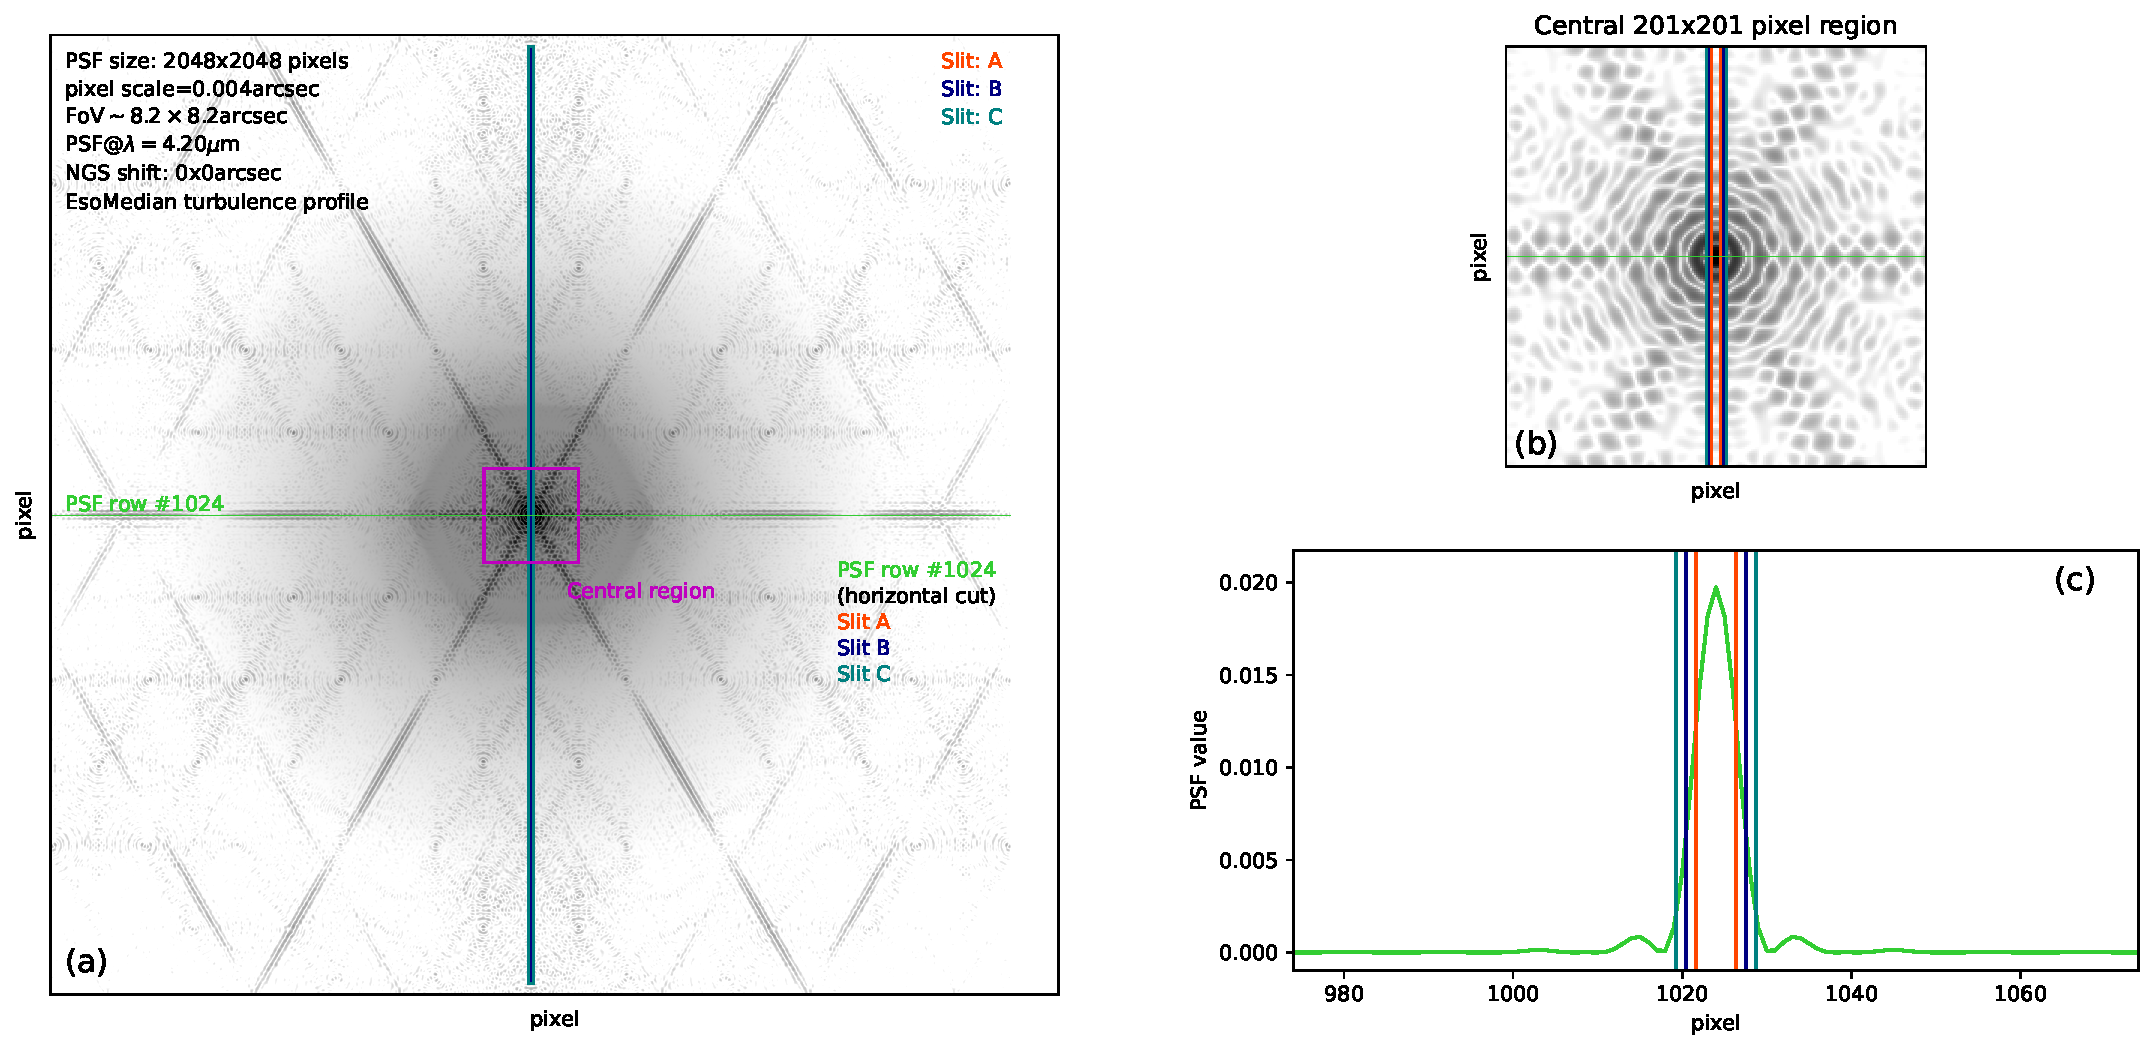
\includegraphics[width=1.0\linewidth]{figures/LSS_CrtAlg_files/SCAOPSF_L-band_4.20mum_slits_ABC_0x0_shift.pdf}
  \caption{Panel (a): \ac{SCAO}-\ac{PSF} at $4.20\,\mu$m with overlaid slits $A$, $B$, and $C$; Panel (b): Zoom to central region shown in panel (a); Panel (c): Central \ac{PSF} peak at row \#1024 with the limits of the three respective slits $A$, $B$, and $C$.}
  \label{fig:scaopsfslits}
\end{figure}

\begin{figure}[ht!]
  \centering
  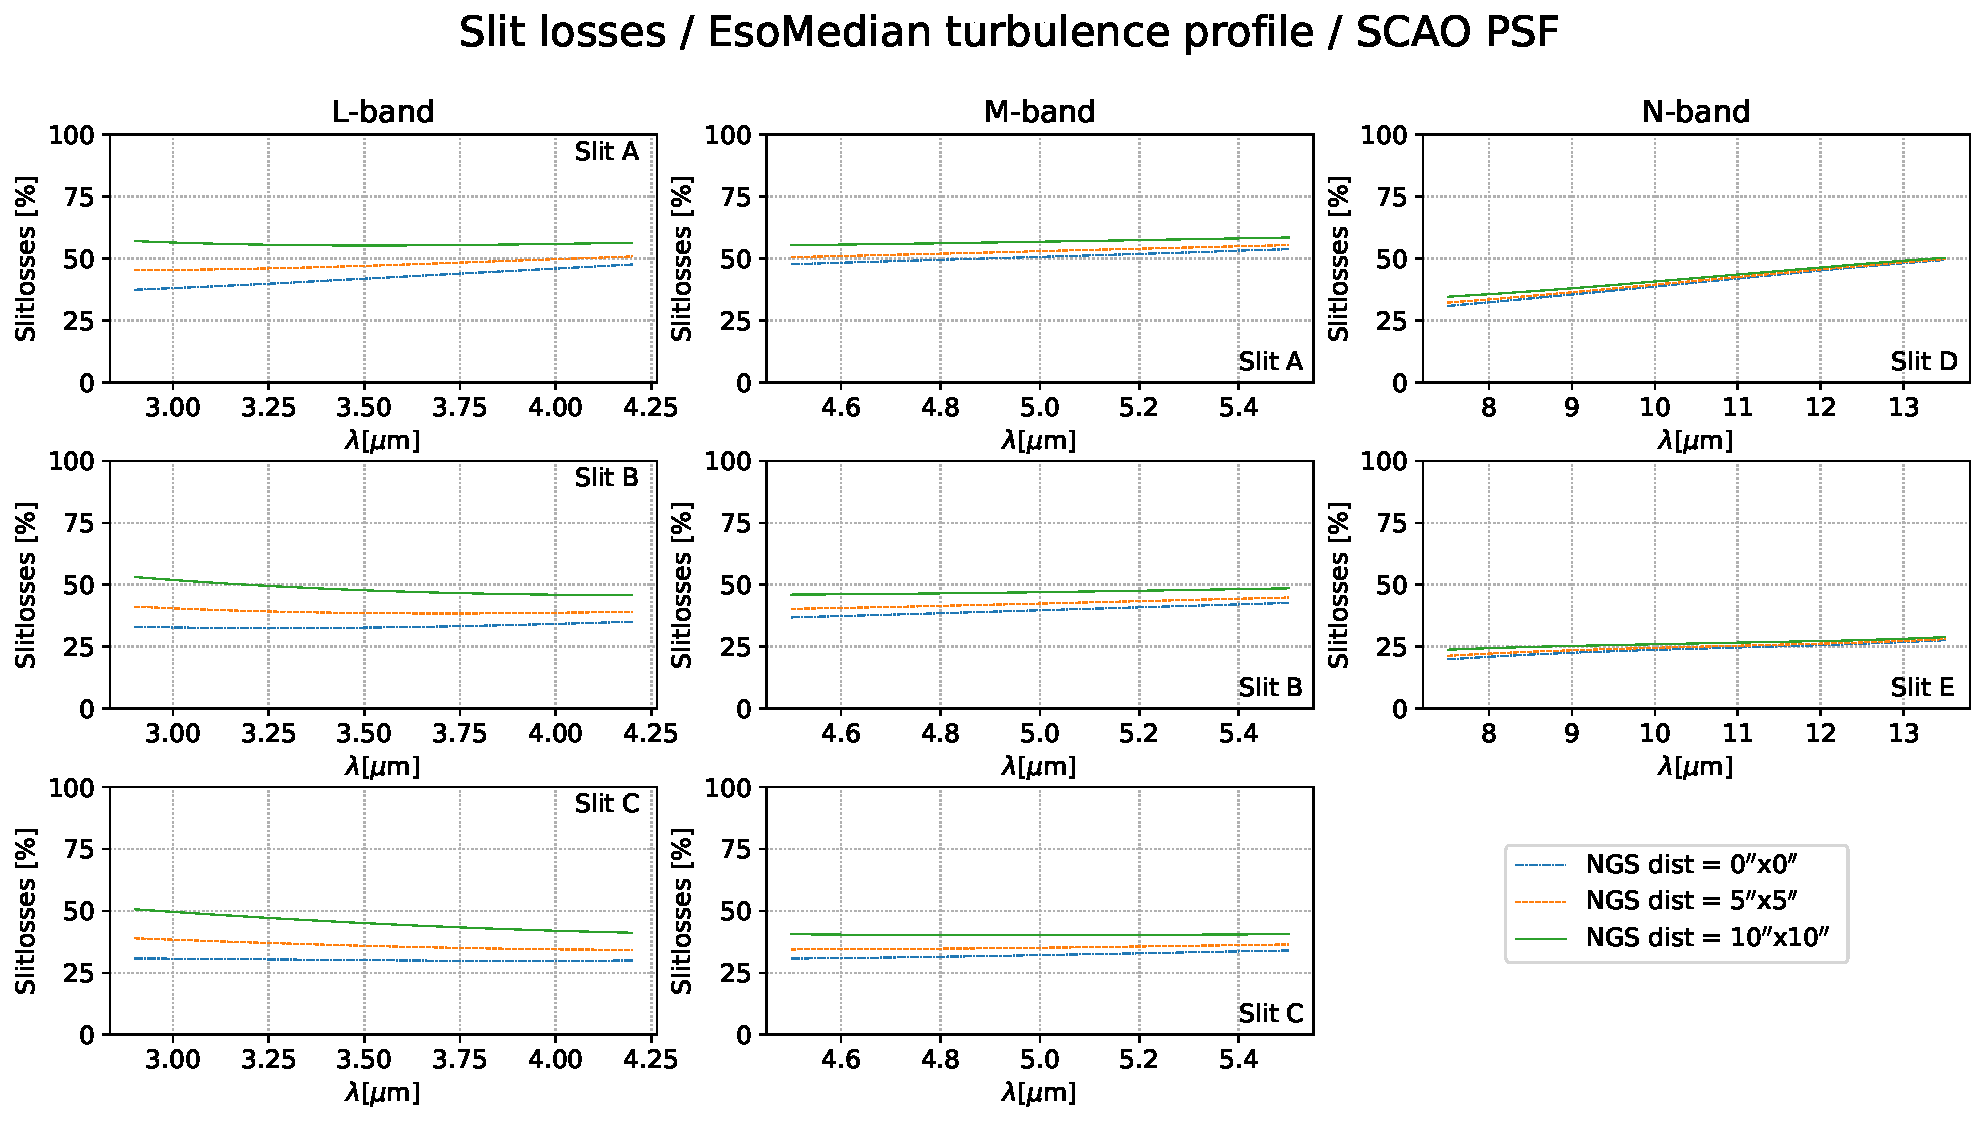
\includegraphics[width=1.0\linewidth]{figures/LSS_CrtAlg_files/METIS_slitlosses.pdf}
  \caption{$L$, $M$, and $N$-band slit losses as function of the wavelengths for all slits.}
  \label{fig:slitlosses}
\end{figure}

\begin{figure}[ht!]
  \centering
  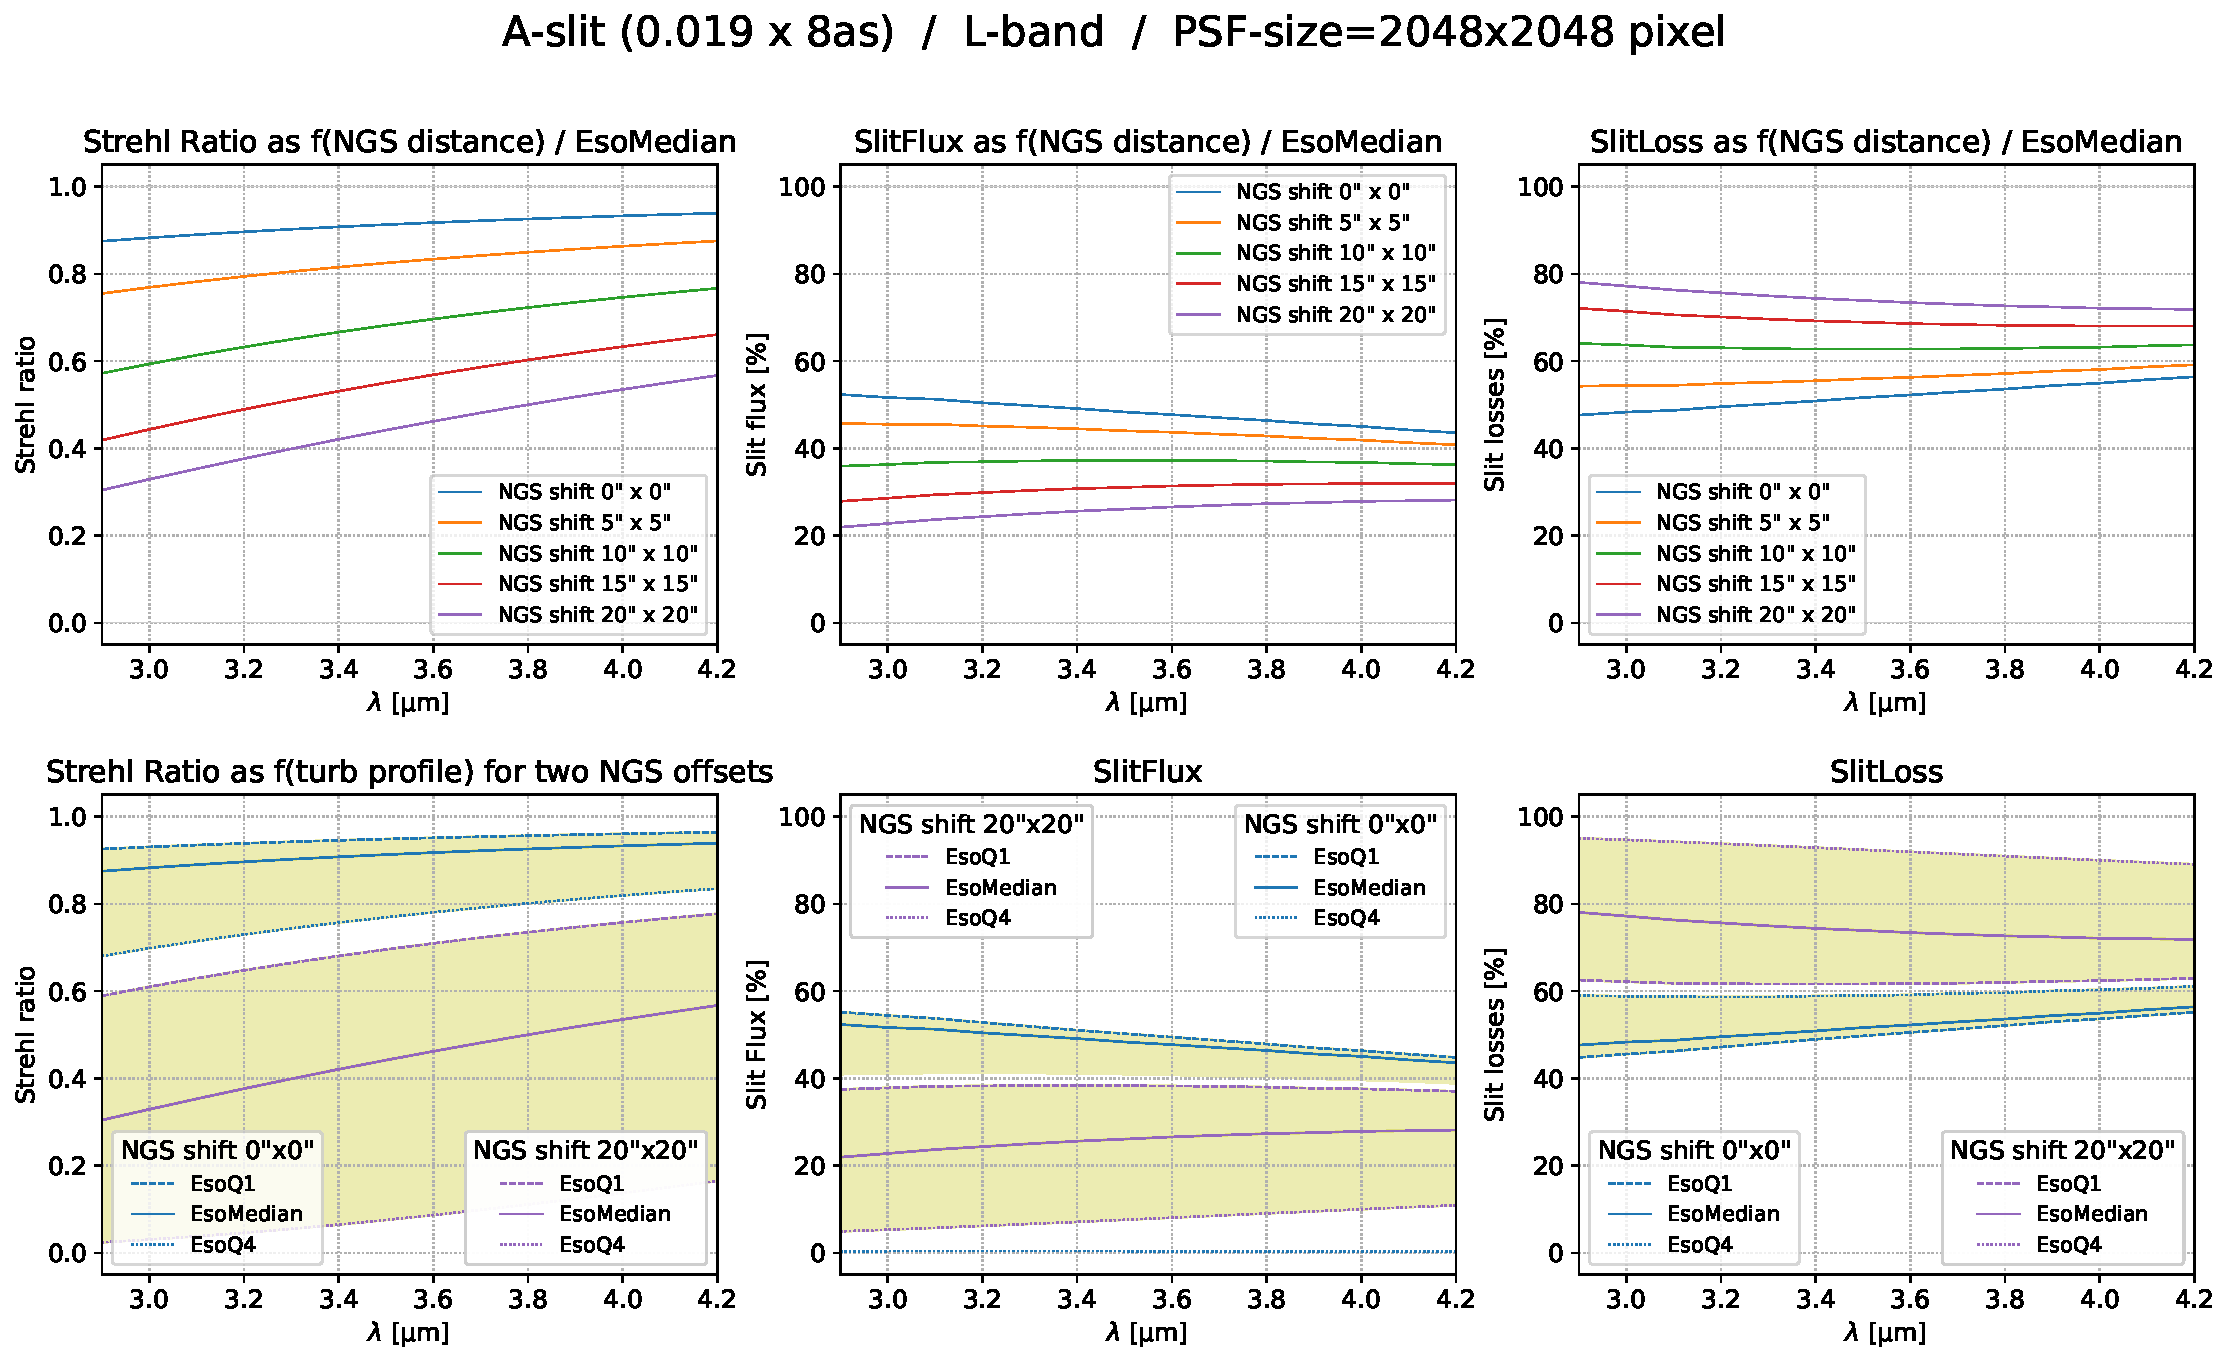
\includegraphics[width=1.0\linewidth]{figures/LSS_CrtAlg_files/SCAO_psf_prop_A_L_ALL.pdf}
  \caption{TBD}
  \label{fig:psf_overview}
\end{figure}


%\paragraph{Spectral resolving power}
%We first estimate the spectral resolving power of the \ac{LSS} mode for the different slits incorporated in the spectrograph. More fancy text to follow \textit{Maybe that part should go somewhere else....?}\cite{METIS-system_analysis}
%\begin{table}
%\begin{center}
%\begin{tabular}{c|cccc|cc|cc}
%Band & $\lambda_\textrm{min}$ & $\lambda_\textrm{cent}$ & $\lambda_\textrm{max}$ & $\Delta\lambda$  & $\lambda_\textrm{min}$ y-Pos & %$\lambda_\textrm{min}$ y-Pos & Dispersion & Dispersion \\
% & [$\mu$m] & [$\mu$m] & [$\mu$m]& on chip [$\mu$m] & on chip [mm] & on chip [mm] & [$\mu$m/mm] & [$\mu$m/pixel]\\
%\hline
%L & 2.9 & 3.55 & 4.2 & 1.300 & 17.856 & -16.704 & 3.762e-02 & 6.771e-04 \\
%M & 4.5 & 4.85 & 5.2 & 0.700 & 17.856 & -16.704 & 2.025e-02 & 3.646e-04 \\
%N & 7.5 & 10.5 & 13.5 & 6.000 & -18.801 & 16.911 & 1.680e-01 & 3.024e-03 \\
%\end{tabular}
%\caption{Spectral dispersion of the long-slit spectrograph in all three bands\label{tab:bands_specres1}}
%\end{center}
%\end{table}

%\begin{table}
%\begin{center}
%\begin{tabular}{c|cc|ccc|ccc}
% & & & proj. Slit & & & & & \\
%Slit & Width$^a$ & Length$^a$ & $L$-band & $M$-band & $N$-band & $L$-band & $M$-band & $N$-band \\
%ID & [mas] & [mas] & [pixel] & [pixel] & [pixel] & Resolution$^b$ & Resolution$^b$ & Resolution$^b$ \\
%\hline
%Slit A & 19.0 & 8000.0 & 2.352e-03 & 1.266e-03 & 8.621e-03 & 1509 & 3830 & 1218 \\
%Slit B & 28.6 & 8000.0 & 3.540e-03 & 1.906e-03 & 1.298e-02 & 1003 & 2544 & 809 \\
%Slit C & 38.1 & 8000.0 & 4.716e-03 & 2.539e-03 & 1.729e-02 & 752 & 1910 & 608 \\
%Slit D & 57.1 & 8000.0 & 7.068e-03 & 3.806e-03 & 2.591e-02 & 502 & 1274 & 405 \\
%Slit E & 114.2 & 8000.0 & 1.414e-02 & 7.612e-03 & 5.182e-02 & 251 & 637 & 203 \\
%\end{tabular}
%\caption{Estimate of the LSS spectral resolving power in all three bands with respect to the different slits;\newline $^a$ from% Tab.~4-2 in~\cite{METIS-system_analysis} \newline $^b$ at $\lambda_\textrm{cent}$ (see Tab.~\ref{tab:bands_specres1})%\label{tab:bands_specres2}}
%\end{center}
%\end{table}


%-----------------------------------------------------------------------------------------
%\subsubsection{Spectroscopic flux calibration strategy for the LSS}\label{ssec:fluxcal}


%\textcolor{red}{TBD: slit flux losses due to PSF (cf. MICADO)?????}




%-----------------------------------------------------------------------------------------
\subsubsection{Object extraction and faint object spectroscopy}\label{sec:fospectro}
The object spectra will be extracted using the optimal extraction described by~\cite{pis21} in order to maximized the \ac{SNR}. 
Faint objects will lead to additional requirements for the observation and the data reduction. For the target acquisition a blind offset from a reference source might become necessary in case the actual object cannot be detected directly. For the data reduction, manual interaction with the user is expected to be necessary to define the target position along the slit since automatic object detection algorithms (e.g. optimal extraction %\cite{hor86}) 
rely on a certain \ac{SNR}. This will be implemented as interactive actor in Reflex (or ESO-DPS).